\chapter{Staggered fermions}\index{fermion!staggered}

In this section we work in a free theory to simplify the notation.
In the interacting theory, each spinor will have a link attached to it
originating at the same point, and the Dirac indices that we will
manipulate commute with these links, so the derivation will be the same.
This follows parts of Section 10.1 in Gattringer and
Lang~\cite{gattringer_quantum_2010} and Section 4.4 in
Rothe~\cite{rothe_lattice_2005}.

We saw before that the doubling problem could
be alleviated by adding a Wilson term of the form
\begin{equation}
  \frac{1}{a}\sum_\mu\id\big(1-\cos(p_\mu a)\big).
\end{equation}
Writing this as exponentials, and doing the Fourier back transformation,
we can express this as
\begin{equation}
  a\sum_{\mu=1}^4\frac{1}{2a^2}
\left(2\delta_{x,y}-\delta_{x,y-a\hat{\mu}}-\delta_{x,y+a\hat{\mu}}\right).
\end{equation}
In this form, one clearly sees that the Wilson term vanishes in the
naive continuum limit like $a$. Moreover it has the form of a
discretized $\partial_\mu\partial_\mu$. A drawback of this term,
however, is that it breaks $\SU_A(N_f)\times\U_A(1)$ explicitly
because the Wilson term commutes with $\gamma_5$.

For some calculations one may desire not to break this symmetry entirely,
in particular when one is investigating phenomena closely related to
chiral symmetry. This motivates other possible fermion discretizations
that remove doublers. {\it Staggered fermions} will remove some of the 
unphysical doublers, while keeping a remnant of this axial symmetry intact. 
This is accomplished by redistributing the quark degrees of freedom over
the lattice in such a way that the spacing between each degree of freedom
doubles, thereby doubling the effective lattice spacing, and hence
reducing the size of the Brillouin zone. New quarks called {\it tastes}
\index{taste}
will be constructed by linear combinations of these degrees of freedom.

We take as the starting point the naive fermion action
\begin{equation}
 S_F
     =a^4\sum_n\bar{\psi}(n)\left(\sum_{\mu=1}^4\gamma_\mu
       \frac{\psi(n+\hat{\mu})-\psi(n-\hat{\mu})}{2a}
       +m\psi(n)\right).
\end{equation}
In this equation and in what follows I will write the space-time coordinate
as $n$ to make the connection between the space-time coordinate and the
following {\it staggered transformation}
\begin{equation}\begin{aligned}
\psi(n)&=\gamma_1^{n_1}\gamma_2^{n_2}\gamma_3^{n_3}\gamma_4^{n_4}\psi(n)'\\
\bar{\psi}(n)
   &=\bar{\psi}(n)'\gamma_4^{n_4}\gamma_3^{n_3}\gamma_2^{n_2}\gamma_1^{n_1}
\end{aligned}\end{equation}
more clear. 

The fact that these transformed fields come with power of gamma matrices,
along with the fact that the gamma matrices are idempotent, will
diagonalize the naive action in Dirac space. In particular one finds
relationships such as
\begin{equation}
  \bar{\psi}(n)\gamma_4\psi(n+\hat{4})
      =(-1)^{n_1+n_2+n_3}\bar{\psi}(n)'\id\psi(n+\hat{4}),
\end{equation}
which means that in the kinetic part, the gamma matrices are annihilated,
and what remains are scalar {\it staggered phases}\index{staggered phase}
\begin{equation}
   \eta_1(n)=1, ~~~
   \eta_2(n)=(-1)^{n_1}, ~~~
   ...\,, ~~~
   \eta_4(n)=(-1)^{n_1+n_2+n_3}.
\end{equation}
Substituting the staggered fields
into the naive action, we thus find
\begin{equation}\label{eq:SFdiag}
   S_F
     =a^4\sum_n\bar{\psi}(n)'\id\left(\sum_{\mu=1}^4\eta_\mu(n)
       \frac{\psi(n+\hat{\mu})'-\psi(n-\hat{\mu})'}{2a}
       +m\psi(n)'\right),
\end{equation}
which is now diagonal in Dirac space because the gammas are gone.
The Dirac operator of eq. \eqref{eq:SFdiag} represents four copies of
the same equations along its diagonal, so we can throw away three copies
without losing any information. We will call this last, kept copy $\chi$;
another way of looking at this is we keep only one Dirac component.
With this notation, we find a particularly simple form for the staggered
action:
\begin{equation}\label{eq:stagg1}
  S_F^{\rm stag}
     =a^4\sum_n\bar{\chi}(n)\left(\sum_{\mu=1}^4\eta_\mu(n)
       \frac{\chi(n+\hat{\mu})-\chi(n-\hat{\mu})}{2a}
       +m\chi(n)\right)
\end{equation}

Equation \eqref{eq:stagg1} is convenient for simulations because it contains no
Dirac spinors explicitly, but we would like a form that tells us a little
more about the physics. We will now begin to rewrite this equation in such
a way that we see the increase of the effective lattice spacing. The
strategy will be to divide the lattice into disjoint unit hypercubes.
The $\chi$ live on the corners of the hypercubes. New fields $q$ will be 
linear combination of the $\chi$, and their sites will be indexed by 
hypercube number.

To this end, we introduce new vectors $h$ (hypercube) and $s$ (corner) that
are related to the original site vectors by
\begin{equation}\label{eq:hypercubeIndex}
  n_\mu=2h_\mu+s_\mu~~~\text{with}~~~h_\mu\in\{0, 1, ..., N_\mu/2\}
                    ~~~s_\mu\in\{0,1\}.
\end{equation}
Moving in the direction $\mu$, $h_\mu$ counts the hypercube number,
while $s$ is a displacement vector starting at the hypercube's origin.
In this indexing scheme
\begin{equation}
  \eta_\mu(n)=\eta_\mu(2h+s)=\eta_\mu(s)
\end{equation}
because contributions to powers of gamma coming from the hypercubes are
always even, according to eq.~\eqref{eq:hypercubeIndex}.

Next we introduce $\Gamma$, which will serve as the weights in the linear
combination. We define
\begin{equation}
  \Gamma^s=\gamma_1^{s_1}\gamma_2^{s_2}\gamma_3^{s_3}\gamma_4^{s_4}.
\end{equation}
These obey, respectively, orthogonality and completeness 
relations\footnote{The orthogonality relation can be proven using
properties of the Euclidean $\gamma$ matrix, in particular that
$\gamma_\mu=\gamma_\mu^\dagger=\gamma_\mu^{-1}$.} 
\begin{equation}
\frac{1}{4}\tr\left[\Gamma^{s\dagger}\Gamma^{s'}\right]=\delta_{ss'}
~~~~\text{and}~~~~
\frac{1}{4}\sum_s\Gamma_{ba}^{s*}\Gamma_{b'a'}^s=\delta_{aa'}\delta_{bb'}
\end{equation}
Our new quark fields are then (see Fig.~\ref{fig:staggHypercubes})
\begin{equation}\label{eq:staggqdef}
  q(h)_{ab}\equiv\frac{1}{8}\sum_s\Gamma^s_{ab}\chi(2h+s)
~~~~\text{and}~~~~
  \bar{q}(h)_{ab}\equiv\frac{1}{8}\sum_s\bar{\chi}(2h+s)\Gamma^{s*}_{ab}.
\end{equation}
In order to cast the staggered action in terms of $q(h)$, we need to
invert eq.~\eqref{eq:staggqdef}. This can be done using the
orthogonality relation. One obtains
\begin{equation}
  \chi(2h+s)=2\tr\left[\Gamma^{s\dagger}q(h)\right]
  ~~~~\text{and}~~~~
  \bar{\chi}(2h+s)=2\tr\Big[\bar{q}(h)\Gamma^s\Big].
\end{equation}

\begin{figure}[t]
  \centering
  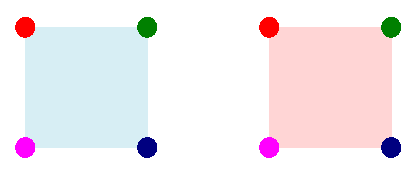
\includegraphics{figs/staggHypercubes.pdf}
  \caption{Example subdivision of one direction into disjoint hypercubes.
           Each hypercube is labeled by $h$, and the field $q(h)$
           associated to the hypercube is a linear combination of the
           $\chi$ fields on the corners, here represented by
           different colors. The effective lattice spacing between
           a $\chi$ of one corner of the blue hypercube and the corresponding
           $\chi$ in the same corner of the red hypercube is $a'=2a$.
           }
  \label{fig:staggHypercubes}
\end{figure}

We are now ready to carry out the substitution. The mass term follows
straightforwardly from the completeness relation. The kinetic term is
difficult, however, because the site offsets mix hypercubes. Therefore
it is crucially important to keep track of which hypercube $\chi$
belongs to. Keeping track of the hypercube will make manifest an $s$
dependence that makes applying the completeness relation not possible,
at least superficially. Gattringer and Lang~\cite{gattringer_quantum_2010}
suggest the following trick: we can shift the site that the first
hypercube starts on by one, which gives equivalent results as the
original hypercube labeling convention, and then average over these
two conventions. I wasn't able to figure this out. 
Rothe~\cite{rothe_lattice_2005} has another strategy, which I was also
not able to follow through. Nevertheless, one should find
\begin{equation}
S_F^{\rm stag}=a'^4\sum_h\Big(m\tr\left[\bar{q}q\right]
+\tr\left[\bar{q}\gamma_\mu\partial_\mu q\right]
-\frac{a'}{2}\tr\left[\bar{q}\gamma_5\Box_\mu q\gamma_\mu\gamma_5\right]\Big)
\end{equation}
where we have an implied summation over $\mu$, we have written
$q=q(h)$, introduced the effective spacing $a'\equiv2a$, and 
the discretized derivatives are
\begin{equation}
  \partial_\mu f(h)\equiv\frac{f(h+\hat{\mu})-f(h-\hat{\mu})}{2a'}
\end{equation}
and
\begin{equation}
  \Box_\mu f(h)\equiv\frac{f(h+\hat{\mu})-2f(h)+f(h-\hat{\mu})}{a'^2}.
\end{equation}

Our final step in the exploration of the staggered action will be to
identify the unphysical fermions. These {\it tastes} are hidden in
\index{taste}
the $q$. This should not be surprising because the $q_{ab}$ have 16
components, but Dirac spinors should have 4. This
tells us each $q$ corresponds to 4 spinors, and we will identify from
the $a$ and $b$ a taste index and Dirac index.
By comparing e.g. the $\tr[\bar{q}q]=\bar{q}_{ab}q_{ba}$ term with
what we expect from the physical, continuum theory, it makes sense
to identify the Dirac index with $b$. Thus our taste spinors are
\begin{equation}
  \psi^{t}(h)_\alpha\equiv q(h)_{\alpha t}~~~~\text{and}~~~~
  \bar{\psi}^{t}(h)_\alpha\equiv \bar{q}(h)_{t\alpha}.
\end{equation}
The staggered fermion action then becomes
\begin{equation}\label{eq:staggPhys}
S_F^{\rm stag}=a'^4\sum_h\left(
m\bar{\psi}^{t}\psi^{t}
+\bar{\psi}^{t}\gamma_\mu\partial_\mu\psi^{t}
-\frac{a'}{2}\bar{\psi}^{t}\gamma_5(\tau_5\tau_\mu)_{tt'}\Box_\mu\psi^{t'}
\right),
\end{equation}
where we have introduced new matrices
\begin{equation}
\tau_\mu\equiv\gamma_\mu^T.
\end{equation}

With the staggered action in the form of eq.~\eqref{eq:staggPhys} we can
begin to discuss some physics. The last term is called the
\index{taste!breaking}
{\it taste-breaking} term. It is similar to the Wilson term, in the
sense that it also represents a second derivative. However unlike
the Wilson term, it allows for interactions between fermions of
\index{taste!mixing}
different taste, i.e. it allows for {\it taste mixing}. If not for
the taste-breaking term, fermions of different taste would be mass-degenerate,
which one sees clearly from the first term. In the naive continuum limit,
this taste breaking terms vanishes like $a$.

The Wilson term broke axial symmetry completely, but in the taste-breaking
term, the remnant $\U_A(1)\times\U_A(1)$ remains. In particular this
term is invariant under transformations
\begin{equation}
\psi'=e^{i\omega}\psi, ~~~~~~
          \bar{\psi}'=\bar{\psi}e^{-i\omega}
\end{equation}
and
\begin{equation}
   \psi'=e^{i\omega\gamma_5\otimes\tau_5}\psi, ~~~~~~
          \bar{\psi}'=\bar{\psi}e^{i\omega\gamma_5\otimes\tau_5}.
\end{equation}
This latter symmetry follows from the fact that $\gamma_5$ commutes through
the taste-breaking term, while $\tau_5$ will pick up a minus sign.
One can identify this symmetry with a subgroup of the axial taste
symmetry group $\SU_A(N_t)$, where $N_t$ is the number of tastes.

At finite lattice spacing, taste mixing lifts the taste mass degeneracy.
One way to get some feeling for taste-breaking effects, then, is to look
at the mass spectrum of staggered fermions. It has been found that these
taste breaking effects can be reduced by improved gauge actions or smearing
\cite{durr_staggered_2004,follana_index_2004}, and in particular smearing
seems to drive masses to 4-fold degeneracy. An intuition for why smearing
might help is as follows: In the interacting theory, each $\chi$ is attached
to links according to its site, and since tastes are linear combinations
of these, it follows that different tastes touch different links. So
the more ``distance" in $\SU(N)$ space between the links, i.e. the more
the links fluctuate, the greater the taste-breaking effects will be.
Since smearing algorithms tend to drive links to more typical values
given their neighbors, they reduce these fluctuations, and hence
the taste-breaking.

We would also like to suppress the effects of unphysical tastes. Absent
taste-breaking, the Dirac operator corresponding to the staggered action
would be block diagonal in taste space, i.e. we would have for 
one physical flavor
\begin{equation}
D^{\rm stag}=\left(\begin{array}{cccc}
            D &   &  &  \\
              & D &  &  \\
              &   & D&  \\
              &   &  & D\\
            \end{array}\right).
\end{equation}
One commonly used strategy to remove the effects of taste-breaking is
\index{rooting}
therefore {\it rooting}. The idea is that $\det D^{\rm stag}$ is
the contribution to the probability distribution from four mass-degenerate
flavors. To isolate one of the flavors, it is sufficient to use
$\det D=(\det D^{\rm stag})^{1/4}$. For two degenerate light flavors
$m_l$ and one heavier flavor $m_s$, i.e. for $N_f=2+1$ fermions, 
one then samples with probability distribution
\begin{equation}
  \dd{\rm P}
    =\dd Ue^{-S_G}(\det D_l^{\rm stag})^{1/2}(\det D_s^{\rm stag})^{1/4}.
\end{equation}

In practice, taste-breaking is present at each lattice spacing, and
therefore it is not clear whether there is some leftover effect of rooting
in the continuum limit. In spite of this danger, people who employ staggered
actions often tend to use rooting anyway. One way to make this step more
justified is to reduce taste-breaking effects. Improved actions such
as the HISQ action, to be discussed in the next section, have greatly
reduced taste-breaking and, reassuringly, results from HISQ actions
seem to agree with experiment.

%\section{Questions}
%\begin{enumerate}
%  \item When can we find a power series expansion for a function of
%        Grassmann numbers?
%  \item Why do we want the integrand to vanish at the boundary?
%\end{enumerate}

\section{Highly improved staggered fermions}\label{sec:HISQ}
\index{action!HISQ}

Highly improved staggered quarks (HISQ) were introduced in 2007 by
Follana {\it et al.} \cite{follana_highly_2007}. This paper summarizes also
some of the history behind staggered quarks, and is written in a generally
friendly way; therefore I encourage the reader to have a look at it.

\index{taste!exchange}
Taste breaking can be thought of through {\it taste exchange}, where
one quark changes its taste by exchanging a virtual gluon with momentum
$p=\pi/a$; a quark with low enough momentum can thereby be pushed into
another corner of the Brillouin zone. See Fig.~\ref{fig:treeLevelTasteExchange}
for a tree-level diagram.
\begin{figure}[t]
  \centering
  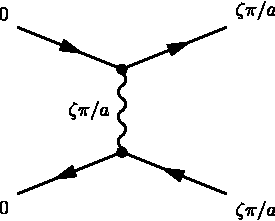
\includegraphics{figs/treelevel.eps}
  \caption{A low-energy quark absorbing a gluon with momentum $\zeta\pi/a$
           can become a quark of another taste. Here $\zeta$ is a vector
           labelling some unphysical corner of the Brillouin zone. Image
           taken from Ref. \cite{follana_highly_2007}.
           }
  \label{fig:treeLevelTasteExchange}
\end{figure}
One goal of HISQ actions, then, is to suppress these processes, which is
done by smearing. Another way to look at taste violations is that they
are a lattice artifact, and so like any other lattice artifact, you would
like to remove its leading order contributions to improve the
approach to the continuum limit. Along this vein, another improvement
made by HISQ is to reduce lattice artifacts from the derivative discretization.

The basic strategy of HISQ can be summarized as:
\begin{enumerate}
  \item Improve finite difference derivatives by 
        \vspace{-1mm}
        \begin{equation*}
         \partial_\mu\to\partial_\mu-\frac{a^2}{6}(1+\epsilon)\partial_\mu^3,
        \end{equation*}
        where $\epsilon$ depends on charm physics. Without considering
        charm physics, this is called a {\it Naik term}.\index{Naik term}
  \item Find a smear $U_\mu\to\mathcal{F}_\mu U_\mu$ that vanishes
        for links carrying momentum $\pi/a$. We start with one
        called {\it Fat7}.\index{Fat7 link}
  \item Multiple smearing reduces mass splittings more, so do that.
  \item Remove new $\mathcal{O}(a^2)$ errors introduced by Fat7.
  \item Smearing enhances some one-loop taste exchange processes,
        which can be suppressed by reunitarizing.
\end{enumerate}
Overall the HISQ smear is then
\begin{equation}\label{eq:HISQsmear}
\mathcal{F}^{\rm HISQ}\equiv
\mathcal{F}^{\rm Fat7}_{\rm corr}\mathcal{U}\mathcal{F}^{\rm Fat7},
\end{equation}
where $\mathcal{F}^{\rm Fat7}_{\rm corr}$ has been corrected for the
errors referenced in step 4, and $\mathcal{U}$ is the reunitarization
operator needed for step 5. The HISQ action uses link variables smeared
by eq.~\eqref{eq:HISQsmear}, and its kinetic term uses improved
Naik discretization.
\begin{figure}
  \centering
  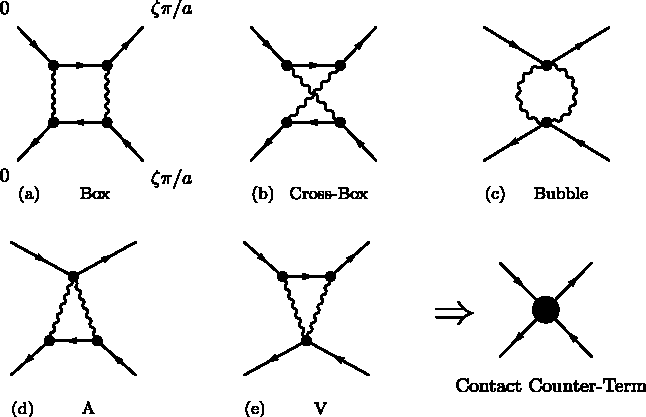
\includegraphics{figs/oneloop.eps}
  \caption{Some example one-loop processes contributing to taste exchange.
           Image taken from Ref. \cite{follana_highly_2007}.
           }
  \label{fig:oneLoopTasteExchange}
\end{figure}
\begin{table}
\begin{tabularx}{\linewidth}{lCCCC} \hline\hline
        & \multicolumn{3}{c}{Unimproved} & Improved \\
         & ASQTAD & HISQ & HYP & ASQTAD \\ \hline
         Avg $d$,$\tilde{d}$ & 0.23 & 0.02 & 0.02 & 0.13\\
        \hline\hline 
\end{tabularx}
\caption{Average coefficients for the taste processes indicated
         in Fig.~\ref{fig:oneLoopTasteExchange} for a few
         types of lattice actions. Columns indicate whether the
         gluons are improved. Excerpt from Table II of
         Ref. \cite{follana_highly_2007}.}
\label{tab:hisq}
\end{table}

To judge how well the HISQ action does, the authors of
Ref.~\cite{follana_highly_2007} calculated several one-loop taste
exchange processes (that fall into several broad categories indicated
in Fig.~\ref{fig:oneLoopTasteExchange}) and determined their coefficients, 
$d$. Table~\ref{tab:hisq} compares the suppression of taste exchange
to other smearing programs. Before HISQ, ASQTAD was a popular dynamical
fermion action, and one sees that, measured in this way, taste effects
in the HISQ action are reduced by an order of magnitude.

\bibliographystyle{unsrtnat}
\bibliography{bibliography}
